
\subsection{Simulation of backgrounds and detector occupancies}
\label{sec:backgrounds}

\subsubsection{Simulated ECal Occupancies and Acceptance}
Description of occupancy and acceptance for the ECal.

\subsubsection{Simulated Tracker Occupancies and Acceptance}
Description of the expected occupancies and acceptance in the SVT from simulation.




\subsection{Trigger rates: ECal and muon detector}
\subsubsection{ECal trigger performance}

The proposed ECal trigger was simulated to test trigger cuts, verify that the trigger has acceptable efficiency for A' events, and verify that the trigger rate is compatible with the HPS DAQ in all running conditions.

Trigger simulation is done in three stages. 
First, various packages are used to simulate beam interactions in the target---details are given in Section \ref{sec:backgrounds}.
The beam background files (equivalent to 100 ms of beam at each energy) are merged into a common StdHep format. 
A' tridents are also simulated using MadGraph. 
Next, the Geant4-based simulations system SLIC \cite{slic} is used to simulate interactions and energy deposition in the magnetic field, tracker, vacuum chamber and ECal. 
Finally, readout and trigger simulation is done using LCSim.
This is a faithful simulation of the detector, DAQ and trigger and has been tested against the actual performance of the test run detector and DAQ.

Trigger rates are shown in Table \ref{tab:trigrates}. These rates are safely under the maximum readout rate of 43 kHz set by the SVT. 
The addition of pions to the 6.6 GeV background sample does not have a significant effect on the trigger rate.

\begin{table}
	\begin{tabular}{|l|r|}
		\hline
		Sample &  Rate (kHz)\\
		\hline
		1.1 GeV	EGS5 				& 33.5 $\pm$ 0.6	\\
		1.1 GeV EGS5+tridents			& 35.5 $\pm$ 0.6	\\
		2.2 GeV	EGS5 				& 22.3 $\pm$ 0.5	\\
		2.2 GeV EGS5+tridents			& 28.3 $\pm$ 0.5	\\
		6.6 GeV	EGS5 				& 5.3 $\pm$ 0.2	\\
		6.6 GeV EGS5+tridents			& 7.4 $\pm$ 0.3	\\
		6.6 GeV EGS5+tridents+pions (FLUKA)	& 7.3 $\pm$ 0.3	\\
		6.6 GeV EGS5+tridents+pions (G4)	& 7.0 $\pm$ 0.3	\\
		\hline
	\end{tabular}
	\caption{ {\small Trigger rates using various background samples. }
	\label{tab:trigrates}}
\end{table}

Trigger efficiency for A' events is defined as the fraction of A' tridents (generated without fiducial cuts) that produce a trigger.

For the performance of the experiment, we are interested in the combined efficiency of the trigger and tracker: the fraction of A' tridents that produce a trigger and leave enough hits in the tracker for a pair of tracks to be reconstructed.
We simulate charge deposition and readout of the tracker (turning off the generation of noise hits), and check each sensor for hits. 
If the DAQ reads out hits in four stereo pairs in each half of the tracker, the event is in the combined acceptance.

Both efficiency values (trigger only, and combined) are shown in Figure \ref{fig:trigeff}. 
Both trigger and tracker acceptances are dominated by the geometric acceptances of the ECal and tracker.

\begin{figure}[ht]
	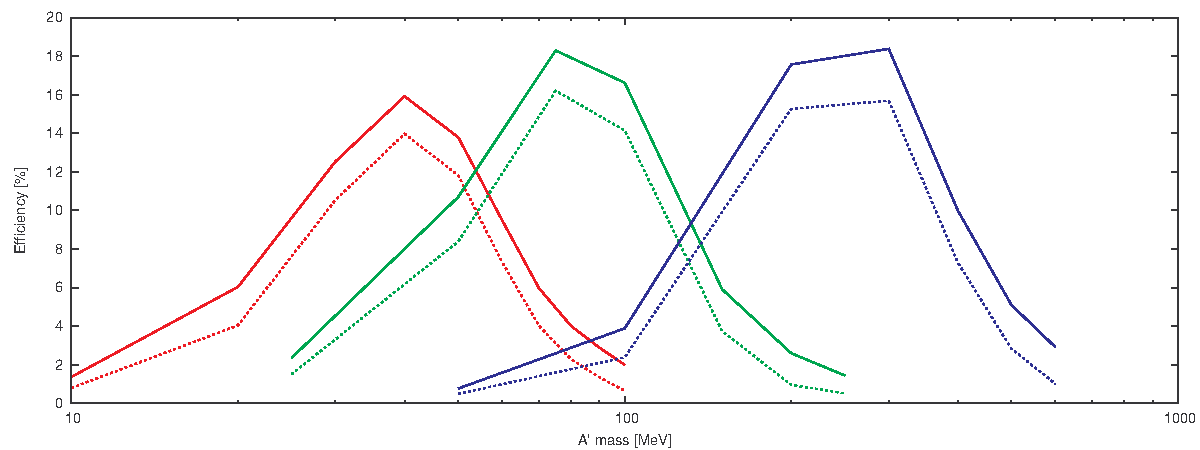
\includegraphics[width=\textwidth]{performance/ap_eff}
	\caption{\small{Trigger efficiency (solid lines) and combined efficiency (dashed lines) as a function of A' mass, at beam energies of 1.1, 2.2 and 6.6 GeV (red, green and blue respectively).}}
	\label{fig:trigeff}
\end{figure}

\subsubsection{Muon trigger performance}

\subsection{Track reconstruction}

\subsection{Cluster reconstruction}

\subsection{Muon identification}

